\section{Arquitetura do Sistema Embarcado}

\subsection{Diagrama}
A distribuição de energia da aeronave segue uma arquitetura centralizada, na qual a bateria atua como fonte de alimentação do sistema. A energia proveniente da bateria é inicialmente encaminhada ao \textit{power module}, responsável por fornecer a tensão regulada de 5V para a controladora de voo Pixhawk 6C Pro. Em paralelo, a energia também é direcionada ao regulador de tensão MH-KC24, utilizado para alimentar o computador de bordo Raspberry Pi 5.

Para o módulo de propulsão, a bateria alimenta a placa de distribuição de energia (PDB), que atua como barramento central para a redistribuição da potência elétrica aos quatro controladores eletrônicos de velocidade (ESCs). Cada ESC converte a energia recebida em sinais trifásicos que acionam os motores, responsáveis pela geração de empuxo da aeronave.

Sendo assim, a estrutura lógica do sistema segue um fluxo simples e funcional:

\begin{figure}[H]
    \centering
    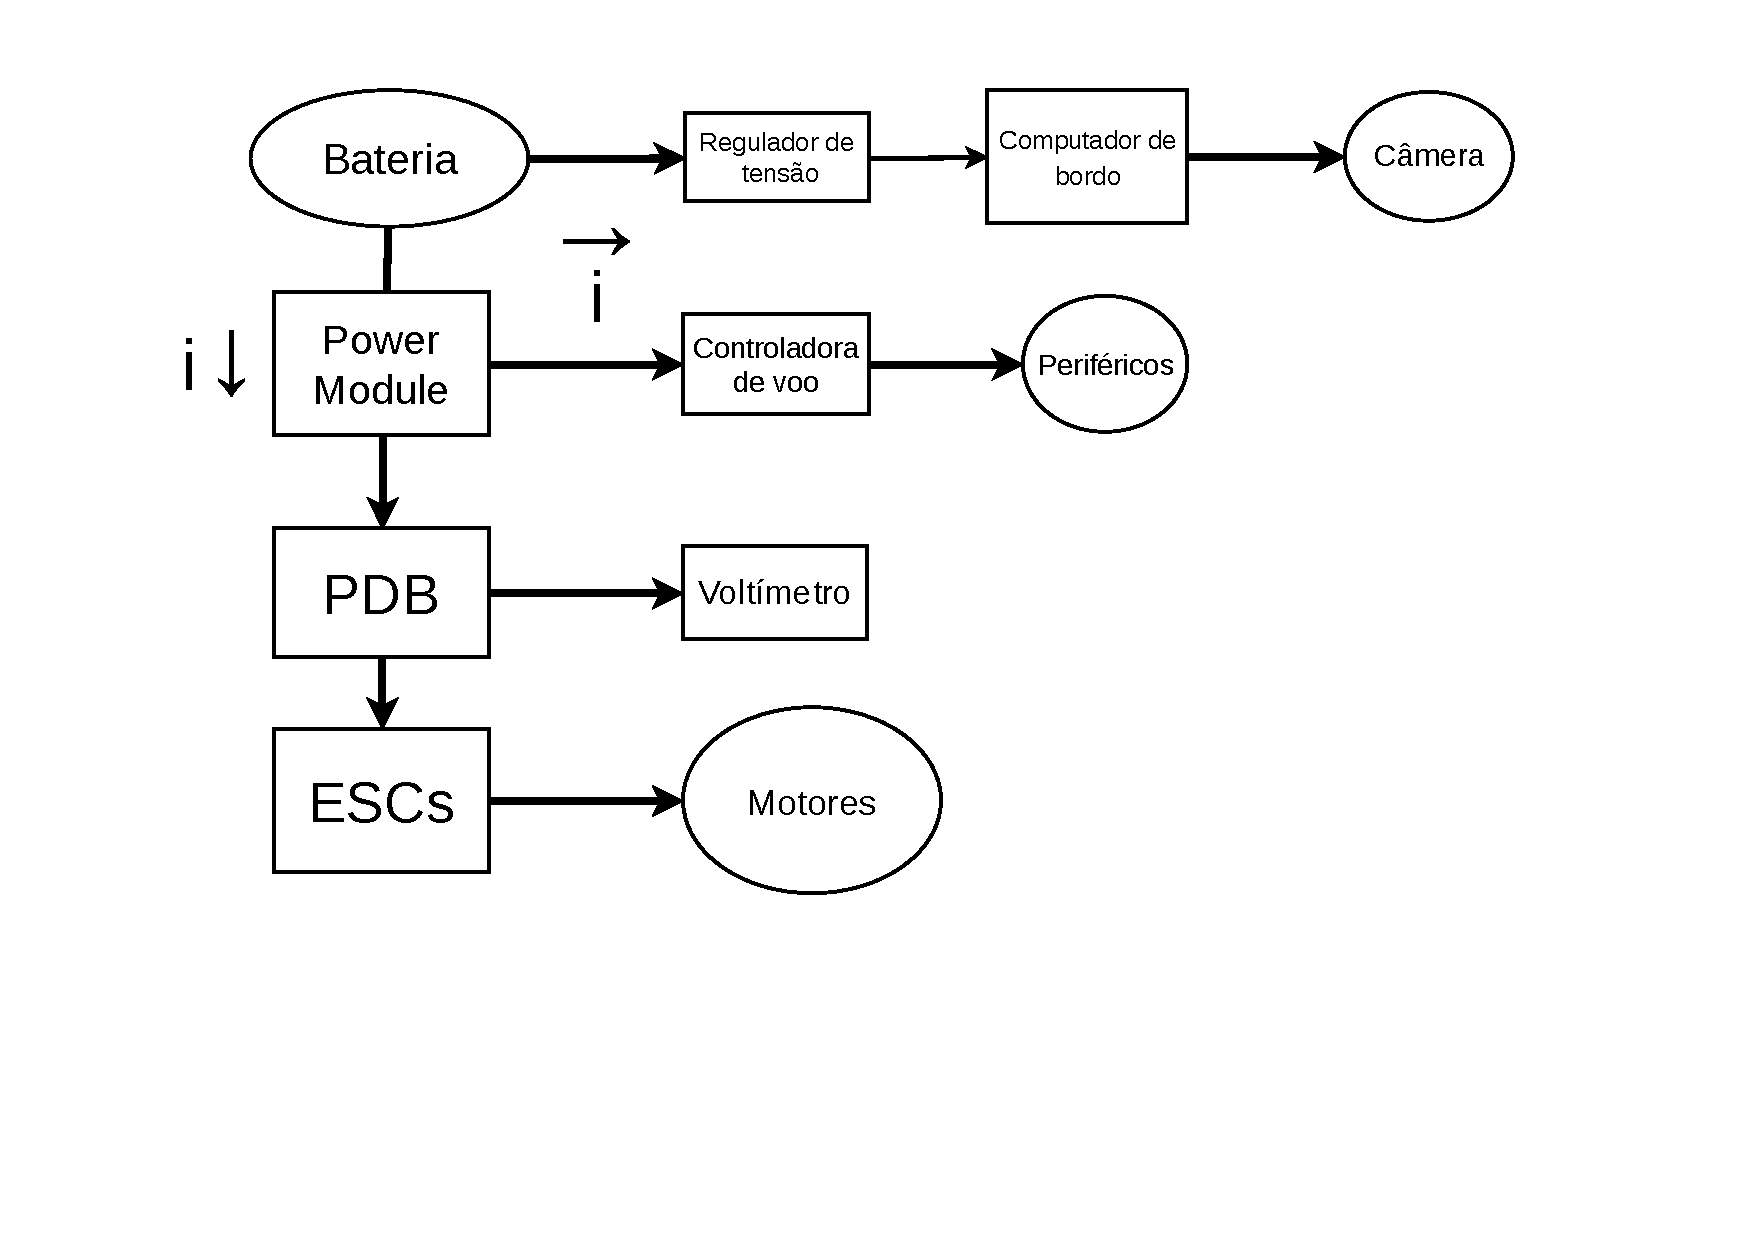
\includegraphics[width=0.65\textwidth]{imagens/FluxoEnergia.pdf}
    \caption{Fluxograma detalhando a distribuição de energia no Logan}
    \label{fig:fluxograma_energia}  
\end{figure}

\subsection{Módulos}

O sistema embarcado da aeronave é estruturado em módulos funcionais responsáveis pela distribuição de energia, controle do voo, aquisição de dados sensoriais e comunicação com a estação de solo. A divisão modular permite maior clareza na integração dos subsistemas, facilita a manutenção e possibilita a validação individual de cada componente durante os testes.

\subsubsection{Propulsão}

O módulo de propulsão é responsável pela geração de empuxo da aeronave. Ele é composto por quatro motores brushless Turnigy D2386/8 acionados por controladores eletrônicos de velocidade (ESCs) Hobbywing Skywalker 40A V2.  

Os ESCs recebem sinais de controle provenientes da controladora de voo e modulam a potência entregue aos motores, permitindo o ajuste dinâmico da rotação e garantindo estabilidade e manobrabilidade durante o voo.

\subsubsection{Alimentação}

O módulo de alimentação realiza o fornecimento e a distribuição da energia elétrica do sistema embarcado. A fonte primária é uma bateria LiPo Turnigy Rapid  4S2P de 8000 mAh 140C, cuja energia é distribuída através de uma placa de distribuição de energia (PDB). A partir desse barramento central, a alimentação é encaminhada aos ESCs e aos módulos eletrônicos sensíveis, incluindo a controladora de voo e o computador de bordo.  

O módulo de potência também permite o monitoramento da tensão e corrente da bateria por meio do \textit{power module}, fornecendo dados utilizados pela controladora para estimativa do estado energético do sistema.

\subsubsection{Navegação}

O módulo de navegação do Logan integra duas camadas principais, responsáveis pela navegabilidade do drone: a camada de controle e a camada de computação. A camada de controle do Logan é centralizada na Pixhawk 6C Pro, enquanto a camada de computação é atribuída ao Raspberry Pi 5. Essa arquitetura já vinha sendo consolidada pela equipe e continua válida por oferecer uma separação funcional eficiente entre estabilização e processamento de alto nível. A Pixhawk é responsável pela navegação básica, controle da atitude, interpretação dos sensores internos e execução das rotinas críticas de voo, enquanto a Raspberry Pi suporta tarefas computacionalmente mais exigentes e logicamente inviáveis para controladora, como visão computacional e lógica de missão. 

A escolha da Pixhawk 6C Pro se sustenta por sua compatibilidade com ArduPilot, ampla disponibilidade de interfaces e integração natural com a estação de solo via Mission Planner. Já a Raspberry Pi 5 fornece margem computacional para processamento de imagem em tempo real, integração com periféricos visuais e implementação de estratégias mais sofisticadas de percepção e decisão. Juntas, essas plataformas compõem o núcleo lógico da autonomia do Logan. 

\subsubsection{Sensoriamento}

O sensoriamento da aeronave combina sensores internos da controladora com sensores externos dedicados à navegação e percepção do ambiente.

A Pixhawk integra sensores inerciais (acelerômetro e giroscópio) como o ICM-42688-P (IMU1) e o BMI055l (IMU2) que são responsáveis pela medição de aceleração e rotação. Além do magnetômetro IST8310 para estimar sua posição relativa no espaço, determinando a orientação e a direção do drone em relação ao norte magnético da Terra e o barômetro MS5611, útil para medir a pressão atmosférica e determinar a altitude da aeronave em relação ao ponto de decolagem. Complementando esse sistema, é utilizado um módulo GPS u-blox NEO-M9N para obtenção de posição geográfica e velocidade horizontal e que com seu magnetômetro embutido, traz redundância sensorial ao módulo. O sistema também incorpora um sensor de fluxo óptico Matek 3901-L0X, utilizado para estimativa de deslocamento relativo em baixa altitude (<7m), e uma câmera Arducam IMX519 conectada ao computador de bordo para permitir navegabilidade autônoma do drone, guiada por visão computacional.

\subsubsection{Comunicação}

A comunicação entre a aeronave e a estação de solo é realizada pelo enlace de telemetria, representado no projeto pelo módulo 3DR Radio V5. Complementarmente, a arquitetura prevê um receptor Futaba R6208SB aliado ao controle transmissor Futaba T8FG, utilizado como camada adicional não-obrigatório de segurança operacional. Essa configuração está alinhada com o regulamento, que estabelece política restrita de conectividade e obriga o uso da estação de solo, tratando-a como parte integrante da operação segura da aeronave. Assim, o enlace de comunicação do Logan é simultaneamente um canal de monitoramento, supervisão, intervenção e validação em voo.

\subsection{Disposição física dos componentes}

A disposição física dos componentes do Logan foi definida de modo a favorecer integração entre módulos, organização do cabeamento e separação entre elementos de potência, controle e sensoriamento. Em 2026, o arranjo adotado também buscou melhorar a acessibilidade para montagem e manutenção, reduzindo a sobreposição entre componentes eletrônicos.

\begin{figure}[H]
    \centering
    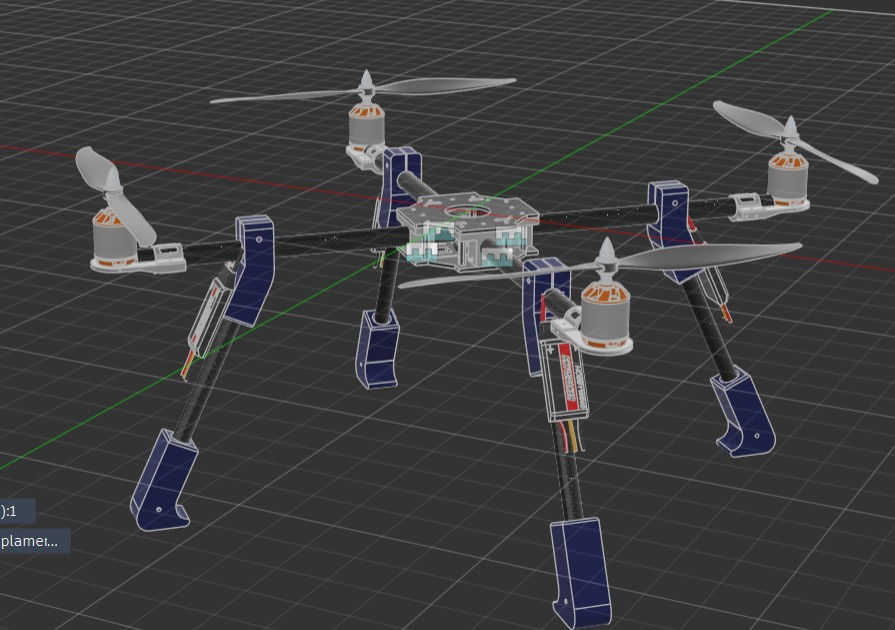
\includegraphics[width=0.5\textwidth]{imagens/frame+motores.jpeg}
    \caption{Vista geral da disposição física dos componentes e do conjunto estrutural do Logan}
    \label{fig:disposicao_geral}
\end{figure}

Na região superior da aeronave foram posicionados os módulos de controle, computação, comunicação e sensoriamento principal, concentrando a Pixhawk, a Raspberry Pi, o GPS, o receptor RC, a antena de telemetria e a câmera. Essa organização aproxima os elementos responsáveis pelo processamento e pela troca de sinais, ao mesmo tempo em que simplifica interconexões e inspeções do sistema.

\begin{figure}[H]
    \centering
    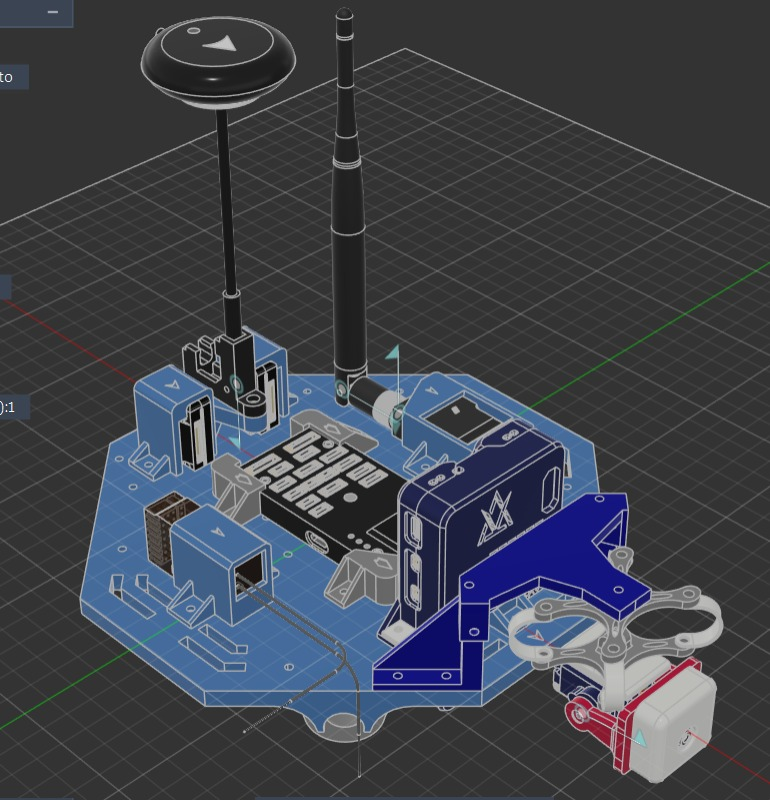
\includegraphics[width=0.5\textwidth]{imagens/superior.jpeg}
    \caption{Disposição dos componentes no suporte superior da aeronave}
    \label{fig:suporte_superior}
\end{figure}

Na região central do frame foi mantida a placa de distribuição de energia, a partir da qual a alimentação é encaminhada para os diferentes módulos da aeronave. Os ESCs foram instalados nos braços, próximos aos motores, enquanto os componentes de maior massa e ligados ao subsistema de alimentação, como bateria, regulador de tensão, voltímetro e sensor de fluxo óptico, foram alocados na parte inferior.

O módulo GPS foi instalado em posição elevada em relação aos demais componentes eletrônicos, aumentando o afastamento físico em relação aos elementos de potência e aos conversores presentes no sistema. Já a bateria e o restante do módulo de alimentação foram montados em uma base inferior ajustável, permitindo acomodação adequada do conjunto embarcado e compatibilização com diferentes configurações da aeronave.

\begin{figure}[H]
    \centering
    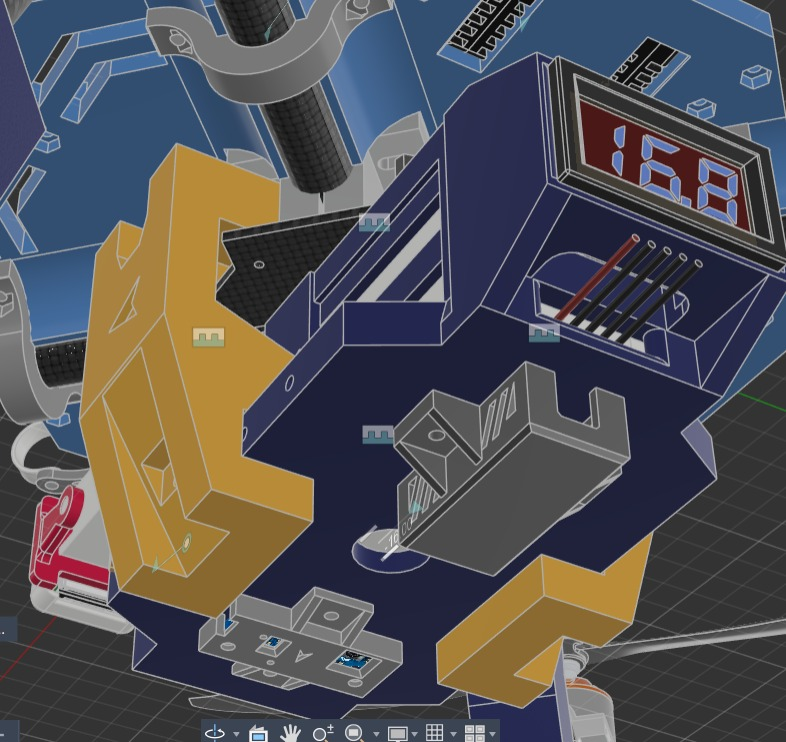
\includegraphics[width=0.5\textwidth]{imagens/inferior.jpeg}
    \caption{Estrutura inferior ajustável destinada à acomodação do subsistema de alimentação. Em amarelo, suportes que permitem que a gaveta (azul) seja ajustável, definindo o CG utilizado em cada configuração do drone}
    \label{fig:suporte_inferior}
\end{figure}

\subsection{Papel do sistema embarcado nas missões}

No Logan, o sistema embarcado atua como a camada responsável por integrar percepção, decisão e atuação ao longo da execução das missões. Sua função não se limita ao controle básico da aeronave, mas envolve a articulação entre controladora de voo, computador de bordo, sensores, enlaces de comunicação e lógica de missão, permitindo que eventos detectados no ambiente sejam convertidos em comandos coerentes de navegação e operação.

A controladora de voo permanece encarregada das funções críticas de estabilização, estimação de estado e execução dos comandos de baixo nível, enquanto o computador de bordo executa algoritmos de visão computacional, processamento de dados e coordenação de comportamentos mais complexos. Essa separação permite que o sistema mantenha robustez nas funções essenciais de voo e, ao mesmo tempo, disponha de capacidade computacional para tarefas como detecção de alvos, interpretação de manômetros, rastreamento visual e suporte à lógica autônoma das missões.

A atuação integrada desses módulos é especialmente relevante no contexto da competição, em que o VANT deve reagir a estímulos do ambiente, manter coerência entre estados operacionais e respeitar restrições de navegação impostas pelo regulamento. Dessa forma, o sistema embarcado do Logan foi estruturado para sustentar uma operação autônoma supervisionada, na qual percepção e ação permanecem conectadas por uma arquitetura única e funcionalmente consistente.
